\chapter{SoC Architecture}\label{chap:socarch}
The supplied ESyLab-SoC plattform is implemented by the \verb=top.vhd=,
which can be found in the \verb=<project root>/soc/top= directory.
Its structure is illustrated by Figure~\ref{fig:socoverview}.
\begin{figure}[htb]
	\centering
	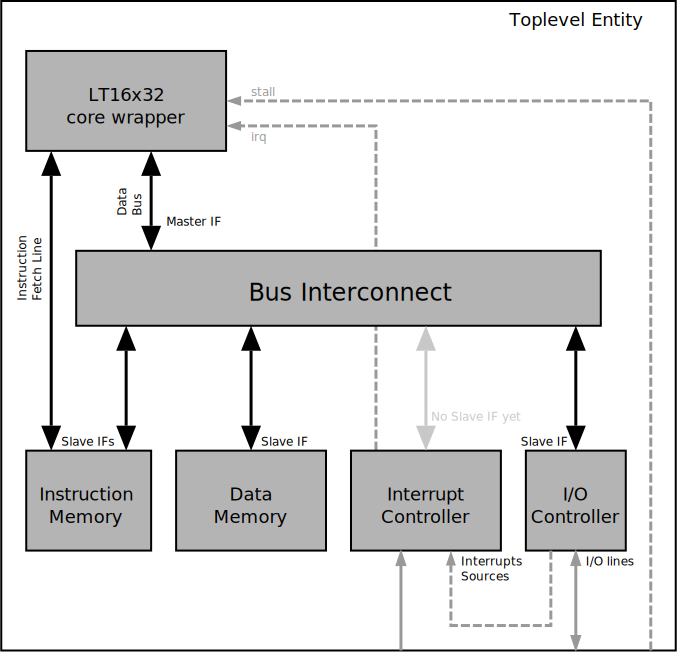
\includegraphics[scale=0.55]{./figures/soc_overview.pdf}
	\caption{Block diagram of the ESyLab-SoC}
	\label{fig:socoverview}
\end{figure}

The interface of the minimal top level entity of the \procname system is shown in Listing~\ref{lst:top_interface}.
\begin{vhdl}[Top Level Entity]{lst:top_interface}
entity lt16soc_top is
generic(
  programfilename : string := "programs/program.ram"
);
port(
  clk		: in  std_logic;
  rst		: in std_logic;
  
  led		: out std_logic_vector(7 downto 0)
);
end entity lt16soc_top;
\end{vhdl}

The inputs \inlinevhdl{clk}, which denote the clock input, and \inlinevhdl{rst}, which is the active high reset, are system-wide signals. 
The minimal system features only one output signal, which is \inlinevhdl{led}.
This signal should be connected to a set of leds and is connected to a generic I/O-controller on the bus.

The individual components of the minimal system are described in the following sections.

\section{Interconnect}
\label{chap:socarch:interconnect}
The system utilizes a synchronous Wishbone bus.
To ease integration of new bus components, a Wishbone bus interconnect component is provided.
The interconnect module currently implements only the synchronous Whisbone protocol.
Its interface is given in Listing~\ref{lst:wb_interconnect_interface}.

\begin{vhdl}[Top Level Entity]{lst:wb_interconnect_interface}
entity wb_intercon is
generic(
  slv_mask_vector : std_logic_vector(0 to NWBSLV-1) := 0;
  mst_mask_vector : std_logic_vector(0 to NWBMST-1) := 0
);
port(
  clk  : in  std_logic;
  rst  : in  std_logic;
  msti : out wb_mst_in_vector;
  msto : in  wb_mst_out_vector;
  slvi : out wb_slv_in_vector;
  slvo : in  wb_slv_out_vector 
);
\end{vhdl}
The system is configured to a certain maximum number of slave and master modules as \inlinevhdl{NWBSLV} and \inlinevhdl{NWBMST} respectively. 
The configuration can be found in \verb=config.vhd=.

These constants are used to define a the length of two generic parameters of the module,
the mask vectors \verb=slv_mask_vector= and \verb=mst_mask_vector=, 
and also define how many elements the input and output arrays have.
As for the mask vectors, as indicated in the \verb=wishbone.vhd= file.
The mask vectors are used to indicate to the interconnect if a module should be connected to the input/output port indicated by the bit position in the mask vector.
A '1' at a position in the mask vector indicates that at the respective position in the the input/output arrays, 
a module should be connected.
A '0' at a position in the mask vector will facilitate that the control logic for that position in the respective input/output array is omitted.

The inputs \inlinevhdl{clk} and \inlinevhdl{rst} are currently not used, but might be in the future when synchronous wishbone transfer is implemented.

The wishbone bus signals are separated in arrays of master and slave signals.
Array of master signals is in the output \inlinevhdl{msti}, which are the inputs to the connected masters, and the input \inlinevhdl{msto}, which are the outputs of the connected master.
Analogously, \inlinevhdl{slvi} and \inlinevhdl{slvo} follow the same principle for the connected slave modules.

\subsection{Integration of new components}
To instantiate a new component in the system, 
a few steps must be undertaken.

\paragraph{The component declaration}%
should not be put in the top level module, 
but in the appropriate package.
This makes the top level module more readable.

\paragraph{The component instantiation}%
in the top level module must be connected to the bus interconnect system.
To do this, the port map must connect its inputs and outputs of its bus interface to a free element of the \verb=slvi= and \verb=slvo= array signals in the top level architecture.
Any element in that vector must obviously only be assigned once.

To select to which of those signals you should connect,
consult the file \verb=soc/lib/config.vhd=.
A number of of slave index constants like shown in Listing~\ref{lst:config_constants} are defined there.
Add your own by adding one to the last defined constant,
then use the defined constant to select the element of the bus slave signal arrays, as illustrated in Listing.~\ref{lst:slave_port_assignment}.

\begin{vhdl}[Slave bus indexes]{lst:config_constants}
-- >> Slave index  <<
constant CFG_MEM : integer := 0; 
constant CFG_LED : integer := CFG_MEM+1;
constant CFG_DMEM : integer := CFG_LED+1;
...
\end{vhdl}
\begin{vhdl}[Slave bus connection]{lst:slave_port_assignment}
... port map( ...
wslvi		=> slvi(CFG_FOO),
wslvo		=> slvo(CFG_FOO)
...
\end{vhdl}

\paragraph{The slave masking vector}%
is a constant which configures the interconnect system to only consider certain slave bus interface elements.
A slave mask vector \verb=slv_mask_vector= is defined in the top level architecture, see Listing~\ref{lst:slave_mask}.
To enable any connection on the interconnect,
the bit in the slave mask vector must be set to '1' at the same position as the targeted elements in the slave connector arrays.

Setting any bit in the slave mask vector to '0' will disable the corresponding connection to the interconnection in the way that the logic to evaluate the inputs is not generated.

\begin{vhdl}[Slave bus indexes]{lst:slave_mask}
architecture RTL of lt16soc_top is
...
constant slv_mask_vector : std_logic_vector(0 to NWBSLV-1) := b"1110_0000_0000_0000";
...
\end{vhdl}

\section{Processor Core Wrapper}
The processor core has a data and instruction memory interface, as per standard Harvard architecture.
The instruction memory interface is unchanged, but the data memory interface is wrapped in a piece of control logic translating the processor interface to wishbone signals and takes care of timing.

\section{Instruction memory}
The instruction memory component is configurable to load a file into its memory during elaboration.
The loaded file needs to contain legal values of the type std\_logic\_vector with a length of 32 characters per line.
If the content of the file is illegal, an error in the elaboration tool will likely occur.

It has two interfaces, one for instruction read access by the processor, one for a read and write access by the Wishbone bus.
The Wishbone interface takes priority over the instruction read.
The whole range of the memory can be written, so care should be exercised when writing to the instruction memory, 
so code or 'constants' are not unintentionally overwritten.
